\chapter{Software testing}
\label{chap:testing}
\section{Overview}
A lot of different standard bodies and writers have defined software testing.
The International Software Testing Qualifications Board (ISTQB) defines software testing
as follows: "The process consisting of all lifecycle activities, both static and
dynamic, concerned with planning, preparation, and evaluation of software products and
related work products; to determine that they satisfy specified requirements,
to demonstrate that they are fit for purpose, and to detect defects." \cite{ctfl_syllabus:2023}

Testing can have different goals, such as getting information about the quality,
supporting decision-making, detecting defects, or preventing defects.
In the process, there are two different approaches: test-as-information-provider
and test-as-quality-accelerant.

In the test-as-information-provider approach, testing is usually executed last in development.
There are independent test teams and separate test phases with fixed release cycles.
Meanwhile, test-as-quality-accelerant follows a test-always strategy.
In the latter approach, testers are quality assistants, and developers
write tests alongside testers.
This allows shorter and more fine-grade releases.
\section{Testing levels}

According to ISTQB, test levels are groups of test activities that are organized
and managed together.
Each test level is an instance of the test process performed concerning
software at a given stage of development, from individual components to complete
systems or, where applicable, system of systems. \cite{ctfl_syllabus:2023}

The ISTQB differentiates the following levels: component (unit), component integration (integration), system, system integration, and acceptance testing. Unit testing focuses on a single component in isolation and is usually performed by developers. Integration testing focuses on testing the interfaces and interactions between components. System tests focus on the overall behavior and capabilities of the entire system or product.

Whittaker et al. show \cite{google:2012} a different approach to test levels used
in Google.
Test levels are defined in execution time; see \autoref{tab:test:levels:google}.
Google uses three different levels: small, medium, and large tests.
Small tests cover a single unit of code in a faked environment.
Medium tests cover two or more interacting features.
Large tests represent real user scenarios and use real user data sources.

\begin{table}
    \centering
    \begin{tabular}{|c c c c|}
        \hline
                    & Small tests   & Medium tests & Large tests            \\
        Time Goals  & $\leq$ 100 ms & $\leq$ 1 sec & As quickly as possible \\
        Time Limits & 1 minute      & 5 minutes    & 1 hour                 \\
        \hline
    \end{tabular}
    \caption{Google's test levels. (Source: \cite{google:2012})}
    \label{tab:test:levels:google}
\end{table}

\section{Test types}
Test types are groups of test activities related to specific quality characteristics, and most of those test activities can be performed at every test level. \cite{ctfl_syllabus:2023}

Common types used in the industry are functional, non-functional, and regression testing.

Functional testing evaluates the functions that a system (or component) should perform. The main objective is to check the functional completeness and correctness of the system.

In Non-functional testing, the goals are to test how well the system behaves. Commonly used software quality characteristics are defined by ISO/IEC 25010 standard\cite{iso_25010:2011}. These characteristics are performance, compatibility, usability, reliability, security, maintainability, and portability. Non-functional tests may need specific test environments.

Regression testing confirms that changes in the codebase did not inject new defects into the functionality. According to ISTQB, performing an impact analysis is advisable to optimize the extent of the regression testing.

\section{Model-based test generation}

Model-based testing (MBT) can best be defined as using models during the testing process \cite{cmbt:syllabus:2015}. Utting et al. \cite{utting2012taxonomy} defined a complete taxonomy for MBT approaches. MBT has two distinct artifacts: a developed model and an adaptor component, which ties the model to the SUT. They defined that the approach has seven major activities (see: \autoref{fig:mbt:taxonomy}):
\begin{enumerate}
    \item model creation
    \item criteria definition
    \item test case generation
    \item creation of the adaptor component
    \item test execution on the SUT
\end{enumerate}
Testers use MBT from unit up to system level testing, but it is used primarily for system and integration testing.

\begin{figure}
    \centering
    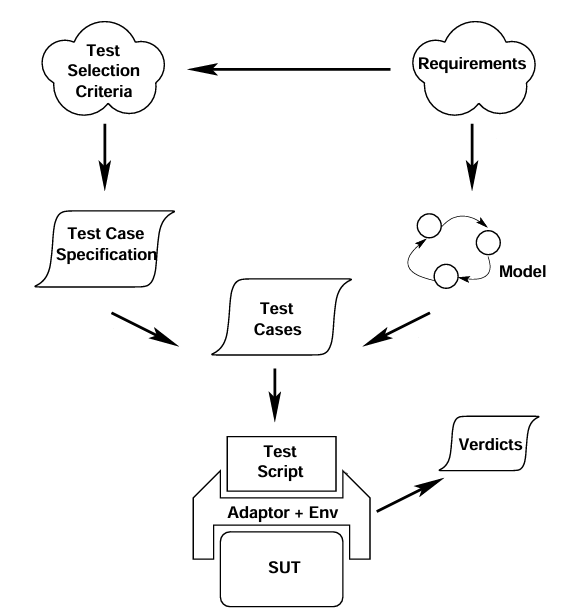
\includegraphics[width=100mm, keepaspectratio]{figures/mbt-taxonomy_uttinger.png}
    \caption{MBT process. (Source: \cite{utting2012taxonomy})}
    \label{fig:mbt:taxonomy}
\end{figure}

Models can best describe the system's intended behavior under test or its environment. Several surveys show that there is only one preferred modeling approach \cite{10.1145/1353673.1353681, mbt-survey:2016, mbt-survey:2019}, but state machine representations are the most popular. Then, state models get transformed into a directed graph. Modeling can be used to abstract different aspects of the SUT (function, data, and communication abstraction)

From the models - based on set criteria - automated tools could generate abstract test cases. The criteria could be in different forms: structural, requirement, or other coverage. Deriving test cases is usually based on random generation or graph search algorithms. Generation could be considered online of offline. In online generation concrete execution starts at the same time as generation. On the other hand, the offline mode can create abstract tests before the adaptor implementation. After the necessary codes are developed, the execution engine could run the offline-generated tests.

Execution engines create concrete test cases in conjunction with the adaptor component from the abstract test cases. The adaptor component wraps the SUT and handles the communication directly. It is used to control and monitor different aspects of the tested system. After the execution, the engine makes a verdict from the SUT responses and reports it back to the QA engineer.

Graphwalker\footnote{\url{https://graphwalker.github.io/}} is a simple but powerful model-based testing tool. It can represent models as directed graphs. Model elements can be either vertexes or edges. Vertexes represent state or validation, and edges represent actions or transitions. The tool integrates a model editor ("studio") and a test execution component. The executor supports many different generation strategies and coverage criteria.

\section{Protocol testing}
Nowadays, academia focuses on proving security issues on protocols and radio. Current studies work on finding vulnerabilities in the protocol itself or its implementation \cite{10.1145/3576915.3623066, 10.1145/3448300.3468287, 10.1145/3448300.3468296, 10.1145/3548606.3560703, 10.1145/3098243.3098254, 10.1145/3597926.3598144, 10.1145/3507657.3528544}.

In terms of IoT testing, a more scalable approach is needed. The literature mentions two types of approaches: simulation and testbeds. Simulation is used when no physical device is available. It is great for validating the functional aspects of a protocol.

The SUT needs to be set up in a realistic environment to evaluate the non-functional properties. Werner-Allen et al. presented a concept for a real wireless network testbed. In their idea, a management layer is introduced for logging and debugging physical devices while users can interact with them. This way, managing and deploying large-scale tests on real hardware is possible\cite{1440979}.

According to Gluhak et al, more and more public testbeds are available\cite{6069710}. More recently, Behnke et al.\cite{10.1145/3368235.3368832} proposed a new hybrid testbed solution that mixes real hardware with optionally simulated nodes.

A survey by Ferriera et al. and Ismail et al.\cite{10.1145/3624032.3624049, 10.3991/ijim.v14i09.13431} showed that model-based techniques were emerging in the realms of IoT testing. Altough MBT is popular, the survey also showed that only a few papers used MBT to generate test cases automatically.

From the papers, I concluded that IoT mainly conducts system-level testing. The industry is using multiple setups to test software, but realistic results come from testing on testbeds. As mentioned above, MBT is an effective technique and is widely available. The deficiency of test case generation from models shows that the industry is not using the full capability of modern MBT tools.